% Created by tikzDevice version 0.11 on 2018-08-26 21:10:20
% !TEX encoding = UTF-8 Unicode
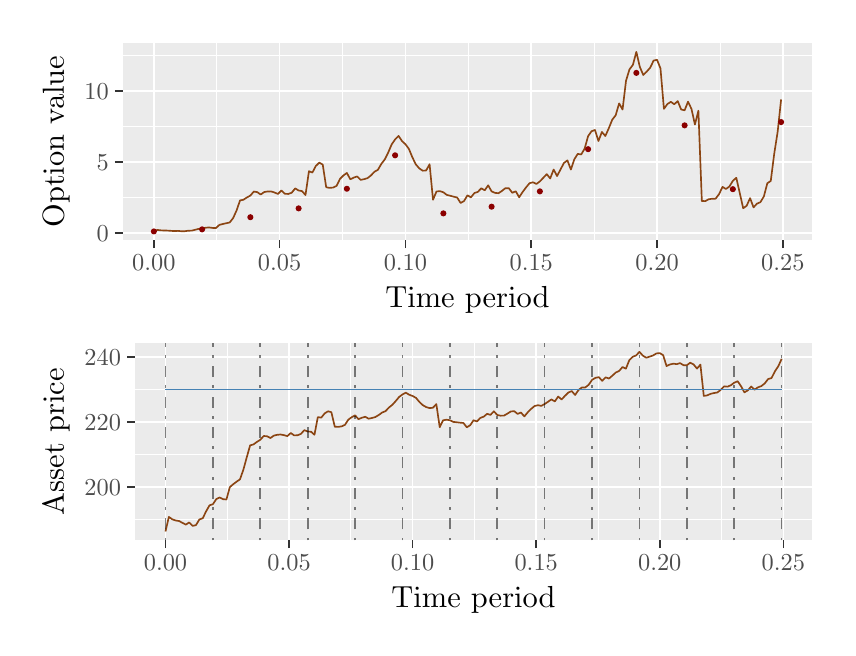
\begin{tikzpicture}[x=1pt,y=1pt]
\definecolor{fillColor}{RGB}{255,255,255}
\path[use as bounding box,fill=fillColor,fill opacity=0.00] (0,0) rectangle (289.08,216.81);
\begin{scope}
\path[clip] (  0.00,108.41) rectangle (289.08,216.81);
\definecolor{drawColor}{RGB}{255,255,255}
\definecolor{fillColor}{RGB}{255,255,255}

\path[draw=drawColor,line width= 0.6pt,line join=round,line cap=round,fill=fillColor] (  0.00,108.41) rectangle (289.08,216.81);
\end{scope}
\begin{scope}
\path[clip] ( 34.27,139.94) rectangle (283.58,211.31);
\definecolor{fillColor}{gray}{0.92}

\path[fill=fillColor] ( 34.27,139.94) rectangle (283.58,211.31);
\definecolor{drawColor}{RGB}{255,255,255}

\path[draw=drawColor,line width= 0.3pt,line join=round] ( 34.27,155.47) --
	(283.58,155.47);

\path[draw=drawColor,line width= 0.3pt,line join=round] ( 34.27,181.18) --
	(283.58,181.18);

\path[draw=drawColor,line width= 0.3pt,line join=round] ( 34.27,206.89) --
	(283.58,206.89);

\path[draw=drawColor,line width= 0.3pt,line join=round] ( 68.33,139.94) --
	( 68.33,211.31);

\path[draw=drawColor,line width= 0.3pt,line join=round] (113.78,139.94) --
	(113.78,211.31);

\path[draw=drawColor,line width= 0.3pt,line join=round] (159.24,139.94) --
	(159.24,211.31);

\path[draw=drawColor,line width= 0.3pt,line join=round] (204.69,139.94) --
	(204.69,211.31);

\path[draw=drawColor,line width= 0.3pt,line join=round] (250.14,139.94) --
	(250.14,211.31);

\path[draw=drawColor,line width= 0.6pt,line join=round] ( 34.27,142.62) --
	(283.58,142.62);

\path[draw=drawColor,line width= 0.6pt,line join=round] ( 34.27,168.33) --
	(283.58,168.33);

\path[draw=drawColor,line width= 0.6pt,line join=round] ( 34.27,194.04) --
	(283.58,194.04);

\path[draw=drawColor,line width= 0.6pt,line join=round] ( 45.60,139.94) --
	( 45.60,211.31);

\path[draw=drawColor,line width= 0.6pt,line join=round] ( 91.05,139.94) --
	( 91.05,211.31);

\path[draw=drawColor,line width= 0.6pt,line join=round] (136.51,139.94) --
	(136.51,211.31);

\path[draw=drawColor,line width= 0.6pt,line join=round] (181.96,139.94) --
	(181.96,211.31);

\path[draw=drawColor,line width= 0.6pt,line join=round] (227.42,139.94) --
	(227.42,211.31);

\path[draw=drawColor,line width= 0.6pt,line join=round] (272.87,139.94) --
	(272.87,211.31);
\definecolor{drawColor}{RGB}{139,69,19}

\path[draw=drawColor,line width= 0.6pt,line join=round] ( 45.60,143.18) --
	( 46.85,143.72) --
	( 48.09,143.58) --
	( 49.34,143.52) --
	( 50.58,143.48) --
	( 51.83,143.39) --
	( 53.07,143.31) --
	( 54.32,143.38) --
	( 55.56,143.24) --
	( 56.81,143.26) --
	( 58.05,143.44) --
	( 59.30,143.47) --
	( 60.54,143.78) --
	( 61.79,144.11) --
	( 63.03,144.17) --
	( 64.28,144.52) --
	( 65.53,144.62) --
	( 66.77,144.45) --
	( 68.02,144.39) --
	( 69.26,145.55) --
	( 70.51,145.86) --
	( 71.75,146.15) --
	( 73.00,146.42) --
	( 74.24,148.00) --
	( 75.49,150.77) --
	( 76.73,154.38) --
	( 77.98,154.63) --
	( 79.22,155.45) --
	( 80.47,156.14) --
	( 81.71,157.59) --
	( 82.96,157.38) --
	( 84.20,156.51) --
	( 85.45,157.40) --
	( 86.70,157.63) --
	( 87.94,157.64) --
	( 89.19,157.25) --
	( 90.43,156.72) --
	( 91.68,157.96) --
	( 92.92,156.79) --
	( 94.17,156.72) --
	( 95.41,157.17) --
	( 96.66,158.73) --
	( 97.90,157.98) --
	( 99.15,157.74) --
	(100.39,156.33) --
	(101.64,164.94) --
	(102.88,164.46) --
	(104.13,166.84) --
	(105.38,168.04) --
	(106.62,167.33) --
	(107.87,159.15) --
	(109.11,158.92) --
	(110.36,159.03) --
	(111.60,159.62) --
	(112.85,162.16) --
	(114.09,163.40) --
	(115.34,164.31) --
	(116.58,162.02) --
	(117.83,162.64) --
	(119.07,163.04) --
	(120.32,161.81) --
	(121.56,162.06) --
	(122.81,162.44) --
	(124.06,163.43) --
	(125.30,164.74) --
	(126.55,165.44) --
	(127.79,167.58) --
	(129.04,169.21) --
	(130.28,171.71) --
	(131.53,174.62) --
	(132.77,176.43) --
	(134.02,177.69) --
	(135.26,175.82) --
	(136.51,174.68) --
	(137.75,173.01) --
	(139.00,169.99) --
	(140.24,167.43) --
	(141.49,165.97) --
	(142.73,165.13) --
	(143.98,165.19) --
	(145.23,167.44) --
	(146.47,154.63) --
	(147.72,157.61) --
	(148.96,157.75) --
	(150.21,157.32) --
	(151.45,156.38) --
	(152.70,156.07) --
	(153.94,155.73) --
	(155.19,155.44) --
	(156.43,153.46) --
	(157.68,154.17) --
	(158.92,156.23) --
	(160.17,155.50) --
	(161.41,157.04) --
	(162.66,157.46) --
	(163.91,158.78) --
	(165.15,158.04) --
	(166.40,159.84) --
	(167.64,157.64) --
	(168.89,157.11) --
	(170.13,156.99) --
	(171.38,157.83) --
	(172.62,158.81) --
	(173.87,158.80) --
	(175.11,157.15) --
	(176.36,157.69) --
	(177.60,155.53) --
	(178.85,157.43) --
	(180.09,159.10) --
	(181.34,160.60) --
	(182.58,160.94) --
	(183.83,160.32) --
	(185.08,161.25) --
	(186.32,162.56) --
	(187.57,163.89) --
	(188.81,162.32) --
	(190.06,165.54) --
	(191.30,163.19) --
	(192.55,165.60) --
	(193.79,167.94) --
	(195.04,168.84) --
	(196.28,165.55) --
	(197.53,169.25) --
	(198.77,171.20) --
	(200.02,170.99) --
	(201.26,173.11) --
	(202.51,177.61) --
	(203.76,179.40) --
	(205.00,179.82) --
	(206.25,175.84) --
	(207.49,179.12) --
	(208.74,177.66) --
	(209.98,180.45) --
	(211.23,183.55) --
	(212.47,185.15) --
	(213.72,189.45) --
	(214.96,187.23) --
	(216.21,197.62) --
	(217.45,201.72) --
	(218.70,203.36) --
	(219.94,208.07) --
	(221.19,202.66) --
	(222.44,199.71) --
	(223.68,200.92) --
	(224.93,202.33) --
	(226.17,204.91) --
	(227.42,205.21) --
	(228.66,202.11) --
	(229.91,187.46) --
	(231.15,189.20) --
	(232.40,190.02) --
	(233.64,189.14) --
	(234.89,190.27) --
	(236.13,187.25) --
	(237.38,186.93) --
	(238.62,190.07) --
	(239.87,187.43) --
	(241.11,181.81) --
	(242.36,186.80) --
	(243.61,154.16) --
	(244.85,154.14) --
	(246.10,154.81) --
	(247.34,155.00) --
	(248.59,155.02) --
	(249.83,156.66) --
	(251.08,159.27) --
	(252.32,158.50) --
	(253.57,159.42) --
	(254.81,161.46) --
	(256.06,162.56) --
	(257.30,157.09) --
	(258.55,151.55) --
	(259.79,152.44) --
	(261.04,155.21) --
	(262.29,151.88) --
	(263.53,153.22) --
	(264.78,153.76) --
	(266.02,155.83) --
	(267.27,160.58) --
	(268.51,161.41) --
	(269.76,171.23) --
	(271.00,179.16) --
	(272.25,190.86);
\definecolor{drawColor}{RGB}{139,0,0}
\definecolor{fillColor}{RGB}{139,0,0}

\path[draw=drawColor,line width= 0.4pt,line join=round,line cap=round,fill=fillColor] ( 45.60,143.18) circle (  0.89);

\path[draw=drawColor,line width= 0.4pt,line join=round,line cap=round,fill=fillColor] ( 63.03,143.93) circle (  0.89);

\path[draw=drawColor,line width= 0.4pt,line join=round,line cap=round,fill=fillColor] ( 80.47,148.32) circle (  0.89);

\path[draw=drawColor,line width= 0.4pt,line join=round,line cap=round,fill=fillColor] ( 97.90,151.51) circle (  0.89);

\path[draw=drawColor,line width= 0.4pt,line join=round,line cap=round,fill=fillColor] (115.34,158.60) circle (  0.89);

\path[draw=drawColor,line width= 0.4pt,line join=round,line cap=round,fill=fillColor] (132.77,170.69) circle (  0.89);

\path[draw=drawColor,line width= 0.4pt,line join=round,line cap=round,fill=fillColor] (150.21,149.70) circle (  0.89);

\path[draw=drawColor,line width= 0.4pt,line join=round,line cap=round,fill=fillColor] (167.64,152.12) circle (  0.89);

\path[draw=drawColor,line width= 0.4pt,line join=round,line cap=round,fill=fillColor] (185.08,157.66) circle (  0.89);

\path[draw=drawColor,line width= 0.4pt,line join=round,line cap=round,fill=fillColor] (202.51,172.90) circle (  0.89);

\path[draw=drawColor,line width= 0.4pt,line join=round,line cap=round,fill=fillColor] (219.94,200.47) circle (  0.89);

\path[draw=drawColor,line width= 0.4pt,line join=round,line cap=round,fill=fillColor] (237.38,181.51) circle (  0.89);

\path[draw=drawColor,line width= 0.4pt,line join=round,line cap=round,fill=fillColor] (254.81,158.45) circle (  0.89);

\path[draw=drawColor,line width= 0.4pt,line join=round,line cap=round,fill=fillColor] (272.25,182.70) circle (  0.89);
\end{scope}
\begin{scope}
\path[clip] (  0.00,  0.00) rectangle (289.08,216.81);
\definecolor{drawColor}{gray}{0.30}

\node[text=drawColor,anchor=base east,inner sep=0pt, outer sep=0pt, scale=  0.88] at ( 29.32,139.59) {0};

\node[text=drawColor,anchor=base east,inner sep=0pt, outer sep=0pt, scale=  0.88] at ( 29.32,165.30) {5};

\node[text=drawColor,anchor=base east,inner sep=0pt, outer sep=0pt, scale=  0.88] at ( 29.32,191.00) {10};
\end{scope}
\begin{scope}
\path[clip] (  0.00,  0.00) rectangle (289.08,216.81);
\definecolor{drawColor}{gray}{0.20}

\path[draw=drawColor,line width= 0.6pt,line join=round] ( 31.52,142.62) --
	( 34.27,142.62);

\path[draw=drawColor,line width= 0.6pt,line join=round] ( 31.52,168.33) --
	( 34.27,168.33);

\path[draw=drawColor,line width= 0.6pt,line join=round] ( 31.52,194.04) --
	( 34.27,194.04);
\end{scope}
\begin{scope}
\path[clip] (  0.00,  0.00) rectangle (289.08,216.81);
\definecolor{drawColor}{gray}{0.20}

\path[draw=drawColor,line width= 0.6pt,line join=round] ( 45.60,137.19) --
	( 45.60,139.94);

\path[draw=drawColor,line width= 0.6pt,line join=round] ( 91.05,137.19) --
	( 91.05,139.94);

\path[draw=drawColor,line width= 0.6pt,line join=round] (136.51,137.19) --
	(136.51,139.94);

\path[draw=drawColor,line width= 0.6pt,line join=round] (181.96,137.19) --
	(181.96,139.94);

\path[draw=drawColor,line width= 0.6pt,line join=round] (227.42,137.19) --
	(227.42,139.94);

\path[draw=drawColor,line width= 0.6pt,line join=round] (272.87,137.19) --
	(272.87,139.94);
\end{scope}
\begin{scope}
\path[clip] (  0.00,  0.00) rectangle (289.08,216.81);
\definecolor{drawColor}{gray}{0.30}

\node[text=drawColor,anchor=base,inner sep=0pt, outer sep=0pt, scale=  0.88] at ( 45.60,128.92) {0.00};

\node[text=drawColor,anchor=base,inner sep=0pt, outer sep=0pt, scale=  0.88] at ( 91.05,128.92) {0.05};

\node[text=drawColor,anchor=base,inner sep=0pt, outer sep=0pt, scale=  0.88] at (136.51,128.92) {0.10};

\node[text=drawColor,anchor=base,inner sep=0pt, outer sep=0pt, scale=  0.88] at (181.96,128.92) {0.15};

\node[text=drawColor,anchor=base,inner sep=0pt, outer sep=0pt, scale=  0.88] at (227.42,128.92) {0.20};

\node[text=drawColor,anchor=base,inner sep=0pt, outer sep=0pt, scale=  0.88] at (272.87,128.92) {0.25};
\end{scope}
\begin{scope}
\path[clip] (  0.00,  0.00) rectangle (289.08,216.81);
\definecolor{drawColor}{RGB}{0,0,0}

\node[text=drawColor,anchor=base,inner sep=0pt, outer sep=0pt, scale=  1.10] at (158.92,115.85) {Time period};
\end{scope}
\begin{scope}
\path[clip] (  0.00,  0.00) rectangle (289.08,216.81);
\definecolor{drawColor}{RGB}{0,0,0}

\node[text=drawColor,rotate= 90.00,anchor=base,inner sep=0pt, outer sep=0pt, scale=  1.10] at ( 13.08,175.62) {Option value};
\end{scope}
\begin{scope}
\path[clip] (  0.00,  0.00) rectangle (289.08,108.41);
\definecolor{drawColor}{RGB}{255,255,255}
\definecolor{fillColor}{RGB}{255,255,255}

\path[draw=drawColor,line width= 0.6pt,line join=round,line cap=round,fill=fillColor] (  0.00,  0.00) rectangle (289.08,108.41);
\end{scope}
\begin{scope}
\path[clip] ( 38.67, 31.53) rectangle (283.58,102.91);
\definecolor{fillColor}{gray}{0.92}

\path[fill=fillColor] ( 38.67, 31.53) rectangle (283.58,102.91);
\definecolor{drawColor}{RGB}{255,255,255}

\path[draw=drawColor,line width= 0.3pt,line join=round] ( 38.67, 39.11) --
	(283.58, 39.11);

\path[draw=drawColor,line width= 0.3pt,line join=round] ( 38.67, 62.60) --
	(283.58, 62.60);

\path[draw=drawColor,line width= 0.3pt,line join=round] ( 38.67, 86.10) --
	(283.58, 86.10);

\path[draw=drawColor,line width= 0.3pt,line join=round] ( 72.13, 31.53) --
	( 72.13,102.91);

\path[draw=drawColor,line width= 0.3pt,line join=round] (116.78, 31.53) --
	(116.78,102.91);

\path[draw=drawColor,line width= 0.3pt,line join=round] (161.43, 31.53) --
	(161.43,102.91);

\path[draw=drawColor,line width= 0.3pt,line join=round] (206.08, 31.53) --
	(206.08,102.91);

\path[draw=drawColor,line width= 0.3pt,line join=round] (250.73, 31.53) --
	(250.73,102.91);

\path[draw=drawColor,line width= 0.6pt,line join=round] ( 38.67, 50.86) --
	(283.58, 50.86);

\path[draw=drawColor,line width= 0.6pt,line join=round] ( 38.67, 74.35) --
	(283.58, 74.35);

\path[draw=drawColor,line width= 0.6pt,line join=round] ( 38.67, 97.85) --
	(283.58, 97.85);

\path[draw=drawColor,line width= 0.6pt,line join=round] ( 49.80, 31.53) --
	( 49.80,102.91);

\path[draw=drawColor,line width= 0.6pt,line join=round] ( 94.45, 31.53) --
	( 94.45,102.91);

\path[draw=drawColor,line width= 0.6pt,line join=round] (139.10, 31.53) --
	(139.10,102.91);

\path[draw=drawColor,line width= 0.6pt,line join=round] (183.76, 31.53) --
	(183.76,102.91);

\path[draw=drawColor,line width= 0.6pt,line join=round] (228.41, 31.53) --
	(228.41,102.91);

\path[draw=drawColor,line width= 0.6pt,line join=round] (273.06, 31.53) --
	(273.06,102.91);
\definecolor{drawColor}{RGB}{139,69,19}

\path[draw=drawColor,line width= 0.6pt,line join=round] ( 49.80, 34.77) --
	( 51.02, 40.02) --
	( 52.25, 39.16) --
	( 53.47, 38.73) --
	( 54.69, 38.54) --
	( 55.92, 37.88) --
	( 57.14, 37.24) --
	( 58.36, 38.03) --
	( 59.59, 36.77) --
	( 60.81, 37.06) --
	( 62.03, 39.08) --
	( 63.26, 39.55) --
	( 64.48, 42.04) --
	( 65.70, 44.19) --
	( 66.93, 44.63) --
	( 68.15, 46.46) --
	( 69.37, 47.04) --
	( 70.60, 46.42) --
	( 71.82, 46.32) --
	( 73.04, 50.78) --
	( 74.27, 51.84) --
	( 75.49, 52.76) --
	( 76.71, 53.58) --
	( 77.94, 57.07) --
	( 79.16, 61.55) --
	( 80.38, 65.87) --
	( 81.61, 66.22) --
	( 82.83, 67.12) --
	( 84.05, 67.88) --
	( 85.28, 69.26) --
	( 86.50, 69.17) --
	( 87.72, 68.52) --
	( 88.95, 69.40) --
	( 90.17, 69.69) --
	( 91.39, 69.80) --
	( 92.62, 69.57) --
	( 93.84, 69.21) --
	( 95.06, 70.36) --
	( 96.29, 69.48) --
	( 97.51, 69.52) --
	( 98.73, 70.01) --
	( 99.96, 71.38) --
	(101.18, 70.89) --
	(102.40, 70.80) --
	(103.63, 69.71) --
	(104.85, 76.09) --
	(106.07, 75.88) --
	(107.30, 77.41) --
	(108.52, 78.19) --
	(109.74, 77.87) --
	(110.97, 72.62) --
	(112.19, 72.55) --
	(113.41, 72.73) --
	(114.64, 73.28) --
	(115.86, 75.15) --
	(117.08, 76.05) --
	(118.31, 76.72) --
	(119.53, 75.35) --
	(120.75, 75.86) --
	(121.98, 76.21) --
	(123.20, 75.51) --
	(124.42, 75.77) --
	(125.65, 76.12) --
	(126.87, 76.85) --
	(128.09, 77.74) --
	(129.32, 78.25) --
	(130.54, 79.55) --
	(131.76, 80.52) --
	(132.99, 81.88) --
	(134.21, 83.36) --
	(135.43, 84.27) --
	(136.66, 84.91) --
	(137.88, 84.16) --
	(139.10, 83.72) --
	(140.33, 83.03) --
	(141.55, 81.56) --
	(142.77, 80.41) --
	(144.00, 79.71) --
	(145.22, 79.34) --
	(146.44, 79.47) --
	(147.67, 80.80) --
	(148.89, 72.43) --
	(150.11, 74.93) --
	(151.34, 75.15) --
	(152.56, 74.95) --
	(153.78, 74.35) --
	(155.01, 74.23) --
	(156.23, 74.08) --
	(157.45, 73.97) --
	(158.68, 72.40) --
	(159.90, 73.16) --
	(161.12, 74.96) --
	(162.35, 74.51) --
	(163.57, 75.81) --
	(164.79, 76.24) --
	(166.02, 77.27) --
	(167.24, 76.89) --
	(168.46, 78.19) --
	(169.69, 76.85) --
	(170.91, 76.60) --
	(172.13, 76.64) --
	(173.36, 77.35) --
	(174.58, 78.12) --
	(175.80, 78.24) --
	(177.03, 77.25) --
	(178.25, 77.75) --
	(179.47, 76.34) --
	(180.70, 77.82) --
	(181.92, 79.04) --
	(183.14, 80.07) --
	(184.37, 80.39) --
	(185.59, 80.15) --
	(186.81, 80.81) --
	(188.04, 81.65) --
	(189.26, 82.47) --
	(190.48, 81.76) --
	(191.71, 83.52) --
	(192.93, 82.45) --
	(194.15, 83.77) --
	(195.38, 84.97) --
	(196.60, 85.48) --
	(197.82, 84.08) --
	(199.05, 85.89) --
	(200.27, 86.79) --
	(201.49, 86.81) --
	(202.72, 87.76) --
	(203.94, 89.55) --
	(205.16, 90.28) --
	(206.39, 90.52) --
	(207.61, 89.18) --
	(208.83, 90.45) --
	(210.06, 90.02) --
	(211.28, 91.07) --
	(212.50, 92.19) --
	(213.73, 92.78) --
	(214.95, 94.18) --
	(216.17, 93.58) --
	(217.40, 96.68) --
	(218.62, 97.87) --
	(219.84, 98.37) --
	(221.07, 99.66) --
	(222.29, 98.29) --
	(223.51, 97.55) --
	(224.74, 97.93) --
	(225.96, 98.36) --
	(227.18, 99.09) --
	(228.41, 99.22) --
	(229.63, 98.46) --
	(230.85, 94.54) --
	(232.08, 95.10) --
	(233.30, 95.40) --
	(234.52, 95.22) --
	(235.75, 95.60) --
	(236.97, 94.84) --
	(238.19, 94.82) --
	(239.42, 95.75) --
	(240.64, 95.10) --
	(241.86, 93.61) --
	(243.09, 95.07) --
	(244.31, 83.75) --
	(245.53, 83.94) --
	(246.76, 84.49) --
	(247.98, 84.78) --
	(249.20, 84.98) --
	(250.43, 85.94) --
	(251.65, 87.21) --
	(252.87, 87.08) --
	(254.10, 87.61) --
	(255.32, 88.52) --
	(256.54, 89.05) --
	(257.77, 87.26) --
	(258.99, 85.04) --
	(260.21, 85.74) --
	(261.44, 87.15) --
	(262.66, 86.01) --
	(263.88, 86.84) --
	(265.11, 87.30) --
	(266.33, 88.26) --
	(267.55, 89.84) --
	(268.78, 90.19) --
	(270.00, 92.60) --
	(271.22, 94.43) --
	(272.45, 97.12);
\definecolor{drawColor}{RGB}{70,130,180}

\path[draw=drawColor,line width= 0.6pt,line join=round] ( 49.80, 86.10) --
	( 51.02, 86.10) --
	( 52.25, 86.10) --
	( 53.47, 86.10) --
	( 54.69, 86.10) --
	( 55.92, 86.10) --
	( 57.14, 86.10) --
	( 58.36, 86.10) --
	( 59.59, 86.10) --
	( 60.81, 86.10) --
	( 62.03, 86.10) --
	( 63.26, 86.10) --
	( 64.48, 86.10) --
	( 65.70, 86.10) --
	( 66.93, 86.10) --
	( 68.15, 86.10) --
	( 69.37, 86.10) --
	( 70.60, 86.10) --
	( 71.82, 86.10) --
	( 73.04, 86.10) --
	( 74.27, 86.10) --
	( 75.49, 86.10) --
	( 76.71, 86.10) --
	( 77.94, 86.10) --
	( 79.16, 86.10) --
	( 80.38, 86.10) --
	( 81.61, 86.10) --
	( 82.83, 86.10) --
	( 84.05, 86.10) --
	( 85.28, 86.10) --
	( 86.50, 86.10) --
	( 87.72, 86.10) --
	( 88.95, 86.10) --
	( 90.17, 86.10) --
	( 91.39, 86.10) --
	( 92.62, 86.10) --
	( 93.84, 86.10) --
	( 95.06, 86.10) --
	( 96.29, 86.10) --
	( 97.51, 86.10) --
	( 98.73, 86.10) --
	( 99.96, 86.10) --
	(101.18, 86.10) --
	(102.40, 86.10) --
	(103.63, 86.10) --
	(104.85, 86.10) --
	(106.07, 86.10) --
	(107.30, 86.10) --
	(108.52, 86.10) --
	(109.74, 86.10) --
	(110.97, 86.10) --
	(112.19, 86.10) --
	(113.41, 86.10) --
	(114.64, 86.10) --
	(115.86, 86.10) --
	(117.08, 86.10) --
	(118.31, 86.10) --
	(119.53, 86.10) --
	(120.75, 86.10) --
	(121.98, 86.10) --
	(123.20, 86.10) --
	(124.42, 86.10) --
	(125.65, 86.10) --
	(126.87, 86.10) --
	(128.09, 86.10) --
	(129.32, 86.10) --
	(130.54, 86.10) --
	(131.76, 86.10) --
	(132.99, 86.10) --
	(134.21, 86.10) --
	(135.43, 86.10) --
	(136.66, 86.10) --
	(137.88, 86.10) --
	(139.10, 86.10) --
	(140.33, 86.10) --
	(141.55, 86.10) --
	(142.77, 86.10) --
	(144.00, 86.10) --
	(145.22, 86.10) --
	(146.44, 86.10) --
	(147.67, 86.10) --
	(148.89, 86.10) --
	(150.11, 86.10) --
	(151.34, 86.10) --
	(152.56, 86.10) --
	(153.78, 86.10) --
	(155.01, 86.10) --
	(156.23, 86.10) --
	(157.45, 86.10) --
	(158.68, 86.10) --
	(159.90, 86.10) --
	(161.12, 86.10) --
	(162.35, 86.10) --
	(163.57, 86.10) --
	(164.79, 86.10) --
	(166.02, 86.10) --
	(167.24, 86.10) --
	(168.46, 86.10) --
	(169.69, 86.10) --
	(170.91, 86.10) --
	(172.13, 86.10) --
	(173.36, 86.10) --
	(174.58, 86.10) --
	(175.80, 86.10) --
	(177.03, 86.10) --
	(178.25, 86.10) --
	(179.47, 86.10) --
	(180.70, 86.10) --
	(181.92, 86.10) --
	(183.14, 86.10) --
	(184.37, 86.10) --
	(185.59, 86.10) --
	(186.81, 86.10) --
	(188.04, 86.10) --
	(189.26, 86.10) --
	(190.48, 86.10) --
	(191.71, 86.10) --
	(192.93, 86.10) --
	(194.15, 86.10) --
	(195.38, 86.10) --
	(196.60, 86.10) --
	(197.82, 86.10) --
	(199.05, 86.10) --
	(200.27, 86.10) --
	(201.49, 86.10) --
	(202.72, 86.10) --
	(203.94, 86.10) --
	(205.16, 86.10) --
	(206.39, 86.10) --
	(207.61, 86.10) --
	(208.83, 86.10) --
	(210.06, 86.10) --
	(211.28, 86.10) --
	(212.50, 86.10) --
	(213.73, 86.10) --
	(214.95, 86.10) --
	(216.17, 86.10) --
	(217.40, 86.10) --
	(218.62, 86.10) --
	(219.84, 86.10) --
	(221.07, 86.10) --
	(222.29, 86.10) --
	(223.51, 86.10) --
	(224.74, 86.10) --
	(225.96, 86.10) --
	(227.18, 86.10) --
	(228.41, 86.10) --
	(229.63, 86.10) --
	(230.85, 86.10) --
	(232.08, 86.10) --
	(233.30, 86.10) --
	(234.52, 86.10) --
	(235.75, 86.10) --
	(236.97, 86.10) --
	(238.19, 86.10) --
	(239.42, 86.10) --
	(240.64, 86.10) --
	(241.86, 86.10) --
	(243.09, 86.10) --
	(244.31, 86.10) --
	(245.53, 86.10) --
	(246.76, 86.10) --
	(247.98, 86.10) --
	(249.20, 86.10) --
	(250.43, 86.10) --
	(251.65, 86.10) --
	(252.87, 86.10) --
	(254.10, 86.10) --
	(255.32, 86.10) --
	(256.54, 86.10) --
	(257.77, 86.10) --
	(258.99, 86.10) --
	(260.21, 86.10) --
	(261.44, 86.10) --
	(262.66, 86.10) --
	(263.88, 86.10) --
	(265.11, 86.10) --
	(266.33, 86.10) --
	(267.55, 86.10) --
	(268.78, 86.10) --
	(270.00, 86.10) --
	(271.22, 86.10) --
	(272.45, 86.10);
\definecolor{drawColor}{RGB}{0,0,0}

\path[draw=drawColor,draw opacity=0.50,line width= 0.6pt,dash pattern=on 1pt off 3pt on 4pt off 3pt ,line join=round] ( 49.80, 31.53) -- ( 49.80,102.91);

\path[draw=drawColor,draw opacity=0.50,line width= 0.6pt,dash pattern=on 1pt off 3pt on 4pt off 3pt ,line join=round] ( 66.93, 31.53) -- ( 66.93,102.91);

\path[draw=drawColor,draw opacity=0.50,line width= 0.6pt,dash pattern=on 1pt off 3pt on 4pt off 3pt ,line join=round] ( 84.05, 31.53) -- ( 84.05,102.91);

\path[draw=drawColor,draw opacity=0.50,line width= 0.6pt,dash pattern=on 1pt off 3pt on 4pt off 3pt ,line join=round] (101.18, 31.53) -- (101.18,102.91);

\path[draw=drawColor,draw opacity=0.50,line width= 0.6pt,dash pattern=on 1pt off 3pt on 4pt off 3pt ,line join=round] (118.31, 31.53) -- (118.31,102.91);

\path[draw=drawColor,draw opacity=0.50,line width= 0.6pt,dash pattern=on 1pt off 3pt on 4pt off 3pt ,line join=round] (135.43, 31.53) -- (135.43,102.91);

\path[draw=drawColor,draw opacity=0.50,line width= 0.6pt,dash pattern=on 1pt off 3pt on 4pt off 3pt ,line join=round] (152.56, 31.53) -- (152.56,102.91);

\path[draw=drawColor,draw opacity=0.50,line width= 0.6pt,dash pattern=on 1pt off 3pt on 4pt off 3pt ,line join=round] (169.69, 31.53) -- (169.69,102.91);

\path[draw=drawColor,draw opacity=0.50,line width= 0.6pt,dash pattern=on 1pt off 3pt on 4pt off 3pt ,line join=round] (186.81, 31.53) -- (186.81,102.91);

\path[draw=drawColor,draw opacity=0.50,line width= 0.6pt,dash pattern=on 1pt off 3pt on 4pt off 3pt ,line join=round] (203.94, 31.53) -- (203.94,102.91);

\path[draw=drawColor,draw opacity=0.50,line width= 0.6pt,dash pattern=on 1pt off 3pt on 4pt off 3pt ,line join=round] (221.07, 31.53) -- (221.07,102.91);

\path[draw=drawColor,draw opacity=0.50,line width= 0.6pt,dash pattern=on 1pt off 3pt on 4pt off 3pt ,line join=round] (238.19, 31.53) -- (238.19,102.91);

\path[draw=drawColor,draw opacity=0.50,line width= 0.6pt,dash pattern=on 1pt off 3pt on 4pt off 3pt ,line join=round] (255.32, 31.53) -- (255.32,102.91);

\path[draw=drawColor,draw opacity=0.50,line width= 0.6pt,dash pattern=on 1pt off 3pt on 4pt off 3pt ,line join=round] (272.45, 31.53) -- (272.45,102.91);
\end{scope}
\begin{scope}
\path[clip] (  0.00,  0.00) rectangle (289.08,216.81);
\definecolor{drawColor}{gray}{0.30}

\node[text=drawColor,anchor=base east,inner sep=0pt, outer sep=0pt, scale=  0.88] at ( 33.72, 47.83) {200};

\node[text=drawColor,anchor=base east,inner sep=0pt, outer sep=0pt, scale=  0.88] at ( 33.72, 71.32) {220};

\node[text=drawColor,anchor=base east,inner sep=0pt, outer sep=0pt, scale=  0.88] at ( 33.72, 94.82) {240};
\end{scope}
\begin{scope}
\path[clip] (  0.00,  0.00) rectangle (289.08,216.81);
\definecolor{drawColor}{gray}{0.20}

\path[draw=drawColor,line width= 0.6pt,line join=round] ( 35.92, 50.86) --
	( 38.67, 50.86);

\path[draw=drawColor,line width= 0.6pt,line join=round] ( 35.92, 74.35) --
	( 38.67, 74.35);

\path[draw=drawColor,line width= 0.6pt,line join=round] ( 35.92, 97.85) --
	( 38.67, 97.85);
\end{scope}
\begin{scope}
\path[clip] (  0.00,  0.00) rectangle (289.08,216.81);
\definecolor{drawColor}{gray}{0.20}

\path[draw=drawColor,line width= 0.6pt,line join=round] ( 49.80, 28.78) --
	( 49.80, 31.53);

\path[draw=drawColor,line width= 0.6pt,line join=round] ( 94.45, 28.78) --
	( 94.45, 31.53);

\path[draw=drawColor,line width= 0.6pt,line join=round] (139.10, 28.78) --
	(139.10, 31.53);

\path[draw=drawColor,line width= 0.6pt,line join=round] (183.76, 28.78) --
	(183.76, 31.53);

\path[draw=drawColor,line width= 0.6pt,line join=round] (228.41, 28.78) --
	(228.41, 31.53);

\path[draw=drawColor,line width= 0.6pt,line join=round] (273.06, 28.78) --
	(273.06, 31.53);
\end{scope}
\begin{scope}
\path[clip] (  0.00,  0.00) rectangle (289.08,216.81);
\definecolor{drawColor}{gray}{0.30}

\node[text=drawColor,anchor=base,inner sep=0pt, outer sep=0pt, scale=  0.88] at ( 49.80, 20.52) {0.00};

\node[text=drawColor,anchor=base,inner sep=0pt, outer sep=0pt, scale=  0.88] at ( 94.45, 20.52) {0.05};

\node[text=drawColor,anchor=base,inner sep=0pt, outer sep=0pt, scale=  0.88] at (139.10, 20.52) {0.10};

\node[text=drawColor,anchor=base,inner sep=0pt, outer sep=0pt, scale=  0.88] at (183.76, 20.52) {0.15};

\node[text=drawColor,anchor=base,inner sep=0pt, outer sep=0pt, scale=  0.88] at (228.41, 20.52) {0.20};

\node[text=drawColor,anchor=base,inner sep=0pt, outer sep=0pt, scale=  0.88] at (273.06, 20.52) {0.25};
\end{scope}
\begin{scope}
\path[clip] (  0.00,  0.00) rectangle (289.08,216.81);
\definecolor{drawColor}{RGB}{0,0,0}

\node[text=drawColor,anchor=base,inner sep=0pt, outer sep=0pt, scale=  1.10] at (161.12,  7.44) {Time period};
\end{scope}
\begin{scope}
\path[clip] (  0.00,  0.00) rectangle (289.08,216.81);
\definecolor{drawColor}{RGB}{0,0,0}

\node[text=drawColor,rotate= 90.00,anchor=base,inner sep=0pt, outer sep=0pt, scale=  1.10] at ( 13.08, 67.22) {Asset price};
\end{scope}
\end{tikzpicture}
